%----------------------------------------------------------------------------------------
% REKENEN MET COMPLEXE GETALLEN. Alle opgaven zijn eigen werk.
%
% Opbouw: Start, leerstof (theorie, werkwijze of uitleg, voorbeeld, korte oefening), en op een
% nieuwe pagina de Opdrachten (door elkaar, stijgende moeilijkheid), Koppel en Test jezelf.
% Labels van dit hoofdstuk beginnen met h1-.
%----------------------------------------------------------------------------------------

\mychapter{1}{Rekenen met complexe getallen}

\lkr{Leerplan B+S'': LPD 38 (complexe getallen voorstellen in het vlak) en LPD 39 (optellen, aftrekken, vermenigvuldigen en delen in cartesische vorm). Het leerplan vraagt $i$ in te voeren als oplossing van $x^2 = -1$, zonder het wortelteken bij een negatief getal, en zonder bewijs aan te geven dat er geen goede ordening op $\C$ bestaat. De rekenregels voor de toegevoegde komen pas in hoofdstuk 2, waar ze nodig zijn.}

De vergelijking $x^2 + 1 = 0$ heeft geen reële oplossing: een kwadraat is nooit negatief. Lange tijd was dat het einde van het verhaal. In de zestiende eeuw ontdekten Italiaanse wiskundigen dat ze bij het oplossen van derdegraadsvergelijkingen soms door een berekening met \textit{vierkantswortels van negatieve getallen} moesten, om op het einde toch een gewoon reëel getal te vinden. Ze rekenden ermee zonder goed te weten wat ze deden.

Vandaag zijn die getallen een stevig deel van de wiskunde. Je voegt aan de reële getallen één nieuw getal $i$ toe, met $i^2 = -1$, en je rekent verder zoals je gewoon bent. Zo krijg je de complexe getallen. Ingenieurs gebruiken ze om wisselstroom te beschrijven, en zonder complexe getallen bestaat er geen kwantummechanica. In dit hoofdstuk leer je ermee rekenen en ze tekenen in een vlak. In hoofdstuk 2 los je er vergelijkingen mee op.

\begin{oefeningen}[Start]
\oef{h1-start-1}

\oef{h1-verken}
\end{oefeningen}

\lkr{Laat oefening \ref{oef:h1-verken} maken vóór de uitleg, na de Opwarmer. Leerlingen rekenen met $i$ zoals met een letter, en vervangen telkens $i^2$ door $-1$. In vraag d vinden ze zelf een oplossing van de vergelijking uit de Opwarmer, die in $\R$ geen oplossingen had. Vraag e bereidt de toegevoegde voor: vergelijk met de wortels in de Opwarmer.}

%========================================================================================
\section{Het getal \texorpdfstring{$i$}{i}}

\subsection{Complexe getallen}

In $\R$ heeft de vergelijking $x^2 = -1$ geen oplossing. We doen wat je in de Verken al gedaan hebt: we nemen aan dat er een getal bestaat met kwadraat $-1$, en we rekenen ermee zoals met een gewoon getal.

\begin{theorie}
De \textbf{\textcolor{accent}{imaginaire eenheid}} $i$ is een getal waarvoor \quad $\formule{i^2 = -1}$

\vspace{1mm}
Een \textbf{\textcolor{accent}{complex getal}} is een getal van de vorm \quad $\formule{z = a + bi}$ \quad met $a, b \in \R$. Dat is de \textbf{\textcolor{accent}{cartesische vorm}} van $z$.

\vspace{1mm}
Het reële getal $a$ is het \textbf{\textcolor{accent}{reëel deel}} $\formule{\Re z}$, het reële getal $b$ het \textbf{\textcolor{accent}{imaginair deel}} $\formule{\Im z}$.
De verzameling van de complexe getallen noteren we $\formule{\C}$.
\end{theorie}

Let op: het imaginair deel van $3 - 5i$ is $-5$, en niet $-5i$. Het reëel en het imaginair deel zijn allebei reële getallen.

Is $b = 0$, dan is $z = a$ een gewoon reëel getal: elk reëel getal is ook een complex getal, dus $\R \subset \C$. Is $a = 0$ en $b \neq 0$, dan heet $z = bi$ \textbf{zuiver imaginair}. Ook $-i$ heeft kwadraat $-1$, want $(-i)^2 = (-1)^2 \cdot i^2 = -1$. De vergelijking $x^2 = -1$ heeft dus twee oplossingen in $\C$: $i$ en $-i$.

We schrijven $i$ nooit als $\sqrt{-1}$. Het wortelteken gebruik je alleen bij een positief getal of 0. Met $\sqrt{-1}$ zou de rekenregel $\sqrt{a} \cdot \sqrt{b} = \sqrt{ab}$ tot onzin leiden: $\sqrt{-1} \cdot \sqrt{-1} = \sqrt{(-1)(-1)} = \sqrt{1} = 1$, terwijl $i \cdot i = -1$.

\voorbeeld{}{Geef het reëel en het imaginair deel van $z_1 = 4 - 7i$, \ $z_2 = 3i$, \ $z_3 = -5$ \ en \ $z_4 = \dfrac{1 - 3i}{2}$.\label{vb:h1-deel}}{%
\uitleg{We schrijven elk getal eerst in de vorm $a + bi$. Dan is $a$ het reëel deel en het getal voor $i$ het imaginair deel, met zijn teken.}
\begin{stappen}
\Re z_1 = 4, \quad \Im z_1 = -7 & Het minteken hoort bij het imaginair deel. \\[1ex]
\Re z_2 = 0, \quad \Im z_2 = 3 & $z_2 = 0 + 3i$ is zuiver imaginair. \\[1ex]
\Re z_3 = -5, \quad \Im z_3 = 0 & $z_3 = -5 + 0i$ is reëel. \\[1ex]
\Re z_4 = \tfrac12, \quad \Im z_4 = -\tfrac32 & Splits de breuk: $z_4 = \tfrac12 - \tfrac32 i$.
\end{stappen}}

\begin{oefeningen}
\oef{h1-deel}
\end{oefeningen}

\subsection{Gelijke complexe getallen}

Kan eenzelfde complex getal op twee manieren in de vorm $a + bi$ staan, met een ander reëel deel? Dan zouden het reëel en het imaginair deel niet goed bepaald zijn. Bij wortels ken je zoiets: $a + b\sqrt2 = c + d\sqrt2$ kan alleen als $a = c$ en $b = d$, omdat $\sqrt2$ geen breuk is. Bij $i$ werkt hetzelfde idee: $i$ is geen reëel getal.

\begin{theorie}
\begin{stelling}{Gelijke complexe getallen}
Twee complexe getallen zijn gelijk als en slechts als hun reële delen gelijk zijn én hun imaginaire delen: voor $a, b, c, d \in \R$ is

\vspace{1mm}
\qquad $\formule{a + bi = c + di \iff a = c \text{ en } b = d}$
\end{stelling}

\begin{bewijs}
Zijn $a = c$ en $b = d$, dan staat links en rechts hetzelfde getal. Stel omgekeerd $a + bi = c + di$. Breng de termen met $i$ naar één lid:
\bewijsregel{(b - d)\,i = c - a .}
Neem aan dat $b \neq d$. Dan mogen we delen door $b - d$, en is $i = \frac{c - a}{b - d}$ een quotiënt van reële getallen, dus zelf een reëel getal. Het kwadraat van een reëel getal is nooit negatief, terwijl $i^2 = -1$. Die tegenspraak toont dat $b = d$. Dan staat er $0 = c - a$, dus ook $a = c$.
\end{bewijs}
\end{theorie}

Het reëel en het imaginair deel van een complex getal liggen dus vast. Een gelijkheid van complexe getallen is eigenlijk een stelsel van twee vergelijkingen met reële getallen: één voor de reële delen, één voor de imaginaire delen.

\voorbeeld{}{Bepaal de reële getallen $x$ en $y$ zodat $(2x - 1) + (y + 3)i = 5 - i$.\label{vb:h1-gelijk}}{%
\uitleg{Beide leden staan in de vorm $a + bi$. We stellen de reële delen gelijk en de imaginaire delen, en lossen de twee vergelijkingen op.}
\begin{stappen}
2x - 1 = 5 \ \Rightarrow \ x = 3 & De reële delen. \\[1ex]
y + 3 = -1 \ \Rightarrow \ y = -4 & De imaginaire delen: het imaginair deel van $5 - i$ is $-1$.
\end{stappen}}

Let op dat $x$ en $y$ reëel moeten zijn. Zonder die voorwaarde mag je niet splitsen: $x + yi = 1$ geeft dan niet alleen $x = 1$ en $y = 0$, maar bijvoorbeeld ook $x = 1 - i$ en $y = 1$, want $(1 - i) + 1 \cdot i = 1$.

\nujij{Bepaal de reële getallen $x$ en $y$ zodat $x + 4i = -2 + 2yi$.}{$x = -2$ en $2y = 4$, dus $y = 2$.}

\begin{oefeningen}
\oef{h1-gelijk}
\end{oefeningen}

%========================================================================================
\section{Het vlak van Gauss}

Een reëel getal stel je voor als een punt op een getallenas. Een complex getal $a + bi$ heeft twee reële getallen nodig, $a$ en $b$: net als een punt in een vlak met een assenstelsel. Die voorstelling is van de Duitse wiskundige Carl Friedrich Gauss, en ze maakt de complexe getallen veel minder geheimzinnig.

\begin{theorie}
\begin{minipage}[t]{.55\linewidth}
\vspace{0pt}
Het complex getal $\formule{a + bi}$ stellen we voor door het punt $\formule{(a, b)}$ in een vlak met een assenstelsel. Dat vlak heet het \textbf{\textcolor{accent}{vlak van Gauss}} of het \textbf{\textcolor{accent}{complexe vlak}}.

\vspace{1mm}
Op de horizontale \textbf{\textcolor{accent}{reële as}} liggen de reële getallen, op de verticale \textbf{\textcolor{accent}{imaginaire as}} de zuiver imaginaire getallen en 0.
\end{minipage}\hfill
\begin{minipage}[t]{.4\linewidth}
\vspace{0pt}
\begin{tikzpicture}[x=.75cm,y=.75cm,font=\small]
  \draw[->,grijs] (-1,0) -- (4.3,0) node[right,text=black,font=\scriptsize] {Re};
  \draw[->,grijs] (0,-1) -- (0,3.4) node[above,text=black,font=\scriptsize] {Im};
  \draw[hulplijn] (3,0) node[below,text=black] {$a$} -- (3,2) -- (0,2) node[left,text=black] {$bi$};
  \draw[vector] (0,0) -- (3,2);
  \cpunt{3}{2}{$a + bi$}
\end{tikzpicture}
\end{minipage}
\end{theorie}

Het punt $(a, b)$ en de pijl van de oorsprong naar dat punt horen allebei bij het getal $a + bi$. Omdat twee complexe getallen alleen gelijk zijn als hun reële en hun imaginaire delen gelijk zijn, hoort bij elk complex getal precies één punt, en omgekeerd. In de volgende sectie zie je waarom de pijl, een vector, handig is.

\voorbeeld{}{Stel de complexe getallen $z_1 = 3 + 2i$, \ $z_2 = -2 + i$, \ $z_3 = -1 - 2i$, \ $z_4 = -3i$ \ en \ $z_5 = 4$ voor in het vlak van Gauss.\label{vb:h1-vlak}}{%
\uitleg{Bij elk getal zoeken we het reëel deel op de horizontale as en het imaginair deel op de verticale as.}
\naast{\begin{minipage}{9cm}
\begin{stappenvrij}{2.6cm}{6cm}
z_1 = 3 + 2i & Drie naar rechts, twee omhoog. \\[1ex]
z_2 = -2 + i & Twee naar links, één omhoog. \\[1ex]
z_3 = -1 - 2i & Eén naar links, twee omlaag. \\[1ex]
z_4 = -3i & Reëel deel 0: op de imaginaire as. \\[1ex]
z_5 = 4 & Imaginair deel 0: op de reële as.
\end{stappenvrij}
\end{minipage}}{\begin{tikzpicture}[x=.66cm,y=.66cm]
  \gauss{-3}{4}{-3}{3}
  \cpunt{3}{2}{$z_1$}
  \cpunt[above left]{-2}{1}{$z_2$}
  \cpunt[left]{-1}{-2}{$z_3$}
  \cpunt[right]{0}{-3}{$z_4$}
  \cpunt[above]{4}{0}{$z_5$}
\end{tikzpicture}}}

\begin{oefeningen}
\oef{h1-vlak}
\end{oefeningen}

\subsection{Groter of kleiner?}

Op de getallenas ligt een groter getal rechts. In het vlak van Gauss bestaat zo'n volgorde niet: je kunt $3 + 2i$ en $-2 + i$ niet zinvol vergelijken. Wiskundigen hebben bewezen dat er geen volgorde op $\C$ bestaat die zich goed gedraagt bij optellen en vermenigvuldigen. Dat bewijs valt buiten deze cursus, maar je ziet het probleem al bij $i$.

In $\R$ geldt: is een getal positief, dan is zijn kwadraat dat ook. Als $i > 0$, dan zou dus ook $i \cdot i > 0$ zijn, en dat zegt $-1 > 0$. Als $i < 0$, dan is $-i > 0$, en dan $(-i) \cdot (-i) > 0$, en dat zegt weer $-1 > 0$. En $i = 0$ kan niet, want $0^2 = 0$. Geen van de drie mogelijkheden werkt. Daarom gebruik je de tekens $<$ en $\leqslant$ nooit tussen complexe getallen. Je mag wel twee moduli vergelijken, zoals je verderop ziet: dat zijn reële getallen.

%========================================================================================
\section{Optellen en aftrekken}

\subsection{De som}

In de Verken heb je $2 + 3i$ en $4 - i$ opgeteld zoals twee veeltermen: de reële delen samen en de imaginaire delen samen. Dat is precies de afspraak.

\begin{theorie}
De \textbf{\textcolor{accent}{som}} van twee complexe getallen: \quad $\formule{(a + bi) + (c + di) = (a + c) + (b + d)i}$
\end{theorie}

In het vlak van Gauss is dat het optellen van vectoren dat je al kent: je telt de coördinaten op. De som $z + w$ is daarom de diagonaal van het parallellogram met zijden $z$ en $w$. Je kunt ook de pijl van $w$ verschuiven tot ze begint in het punt $z$: ze eindigt dan in $z + w$.

\voorbeeld{}{Bereken $z + w$ voor $z = 3 + i$ en $w = -1 + 2i$, en stel de som voor in het vlak van Gauss.\label{vb:h1-som}}{%
\uitleg{We tellen de reële delen op en de imaginaire delen. In de figuur controleren we met het parallellogram.}
\naast{\begin{minipage}{\linewidth}
\begin{stappenvrij}{3.9cm}{4.5cm}
z + w = (3 - 1) + (1 + 2)i & Reëel bij reëel, imaginair bij imaginair. \\
\phantom{z + w} = 2 + 3i &
\end{stappenvrij}

\vspace{1mm}
In de figuur is $z + w$ de diagonaal van het parallellogram met zijden $z$ en $w$. Vanuit $z$ ga je één naar links en twee omhoog, zoals bij $w$, en je komt in $2 + 3i$.
\end{minipage}}{\begin{tikzpicture}[x=.72cm,y=.72cm]
  \gauss{-2}{4}{-1}{3}
  \draw[hulplijn] (3,1) -- (2,3) -- (-1,2);
  \draw[vector] (0,0) -- (3,1);
  \draw[vector] (0,0) -- (-1,2);
  \draw[vector,fel!80!black] (0,0) -- (2,3);
  \cpunt[right]{3}{1}{$z$}
  \cpunt[above left]{-1}{2}{$w$}
  \cpunt[above right]{2}{3}{$z + w$}
\end{tikzpicture}}}

\subsection{Tegengestelde en verschil}

In $\R$ is aftrekken hetzelfde als het tegengestelde optellen: $5 - 3 = 5 + (-3)$. In $\C$ spreken we hetzelfde af.

\begin{theorie}
Het \textbf{\textcolor{accent}{tegengestelde}} van $z = a + bi$ is \quad $\formule{-z = -a - bi}$

\vspace{1mm}
Het \textbf{\textcolor{accent}{verschil}} van twee complexe getallen is \quad $\formule{z - w = z + (-w)}$, \ dus

\vspace{1mm}
\qquad $\formule{(a + bi) - (c + di) = (a - c) + (b - d)i}$
\end{theorie}

Het tegengestelde $-z$ is het spiegelbeeld van $z$ om de oorsprong: beide coördinaten veranderen van teken. En $z + (-z) = 0$, net als in $\R$. Het verschil $z - w$ heeft een mooie betekenis in het vlak: het is de vector van $w$ naar $z$, verschoven tot hij in de oorsprong begint. Want $w + (z - w) = z$: vanuit $w$ kom je met de pijl van $z - w$ in $z$.

\voorbeeld{}{Bereken $z - w$ voor dezelfde $z = 3 + i$ en $w = -1 + 2i$, en stel het verschil voor.\label{vb:h1-verschil}}{%
\uitleg{We trekken de reële delen af en de imaginaire delen. In de figuur zoeken we de pijl van $w$ naar $z$.}
\naast{\begin{minipage}{\linewidth}
\begin{stappenvrij}{3.9cm}{4.5cm}
z - w = (3 + 1) + (1 - 2)i & Een negatief getal aftrekken is het tegengestelde optellen. \\
\phantom{z - w} = 4 - i &
\end{stappenvrij}

\vspace{1mm}
Het tegengestelde $-w = 1 - 2i$ ligt tegenover $w$. Tel je het op bij $z$, dan kom je in $z - w$. De gestippelde pijl van $w$ naar $z$ is even lang en even gericht als die van $0$ naar $z - w$: vier naar rechts en één omlaag.
\end{minipage}}{\begin{tikzpicture}[x=.72cm,y=.72cm]
  \gauss{-2}{4}{-2}{3}
  \draw[vector] (0,0) -- (3,1);
  \draw[vector] (0,0) -- (-1,2);
  \draw[vector,grijs] (0,0) -- (1,-2);
  \draw[vector,fel!80!black] (0,0) -- (4,-1);
  \draw[-{Stealth[length=2mm]},grijs,dashed] (-1,2) -- (3,1);
  \cpunt[right]{3}{1}{$z$}
  \cpunt[above left]{-1}{2}{$w$}
  \cpunt[below right]{1}{-2}{$-w$}
  \cpunt[right]{4}{-1}{$z - w$}
\end{tikzpicture}}}

\subsection{Een reëel veelvoud}

Een complex getal vermenigvuldigen met een reëel getal $r$ doe je zoals bij een veelterm: elke term maal $r$.

\begin{theorie}
Voor een reëel getal $r$ is \quad $\formule{r(a + bi) = ra + rbi}$
\end{theorie}

In het vlak van Gauss is dat het veelvoud van een vector. Beide coördinaten worden met $r$ vermenigvuldigd, dus het punt blijft op de rechte door 0 en $z$. Is $r > 0$, dan wijst $rz$ dezelfde kant op, $r$ keer zo ver. Is $r < 0$, dan wijst $rz$ de andere kant op. Met $r = -1$ vind je het tegengestelde.

\voorbeeld{}{Bereken $2z$, \ $\tfrac12 z$ \ en \ $-z$ voor $z = 2 + i$, en stel ze voor.\label{vb:h1-veelvoud}}{%
\uitleg{De drie opgaven horen samen: ze tonen wat de factor $r$ doet met de pijl. We vermenigvuldigen telkens het reëel en het imaginair deel.}
\naast{\begin{minipage}{9.3cm}
\begin{stappenvrij}{3cm}{6cm}
2z = 4 + 2i & Dezelfde richting, twee keer zo ver. \\[1ex]
\tfrac12 z = 1 + \tfrac12 i & Dezelfde richting, half zo ver. \\[1ex]
-z = -2 - i & Even ver, de andere kant op: het spiegelbeeld om 0.
\end{stappenvrij}

\vspace{1mm}
Alle drie liggen ze op de rechte door $0$ en $z$.
\end{minipage}}{\begin{tikzpicture}[x=.62cm,y=.62cm]
  \gauss{-3}{4}{-2}{2}
  \draw[hulplijn] (-3,-1.5) -- (4.4,2.2);
  \draw[vector,fel!80!black] (0,0) -- (4,2);
  \draw[vector] (0,0) -- (2,1);
  \draw[vector,grijs] (0,0) -- (-2,-1);
  \cpunt[above left]{4}{2}{$2z$}
  \cpunt[below right]{2}{1}{$z$}
  \cpunt[above left]{1}{.5}{$\tfrac12 z$}
  \cpunt[below right]{-2}{-1}{$-z$}
\end{tikzpicture}}}

\begin{werkwijze}
Tel de reële delen op of trek ze af, en doe hetzelfde met de imaginaire delen. Werk een veelvoud eerst uit: $2(3 - i) = 6 - 2i$. Wil je controleren, teken dan de pijlen: een som is de diagonaal van een parallellogram.
\end{werkwijze}

\nujij{Bereken $2z - 3w$ voor $z = 1 - i$ en $w = 2 + i$.}{$2z - 3w = 2 - 2i - 6 - 3i = -4 - 5i$.}

\begin{oefeningen}
\oef{h1-som}

\oef{h1-vectoren}
\end{oefeningen}

%========================================================================================
\section{Vermenigvuldigen}

\subsection{Het product}

Ook vermenigvuldigen doe je zoals bij veeltermen: elke term van de eerste factor maal elke term van de tweede. Het enige nieuwe is dat je $i^2$ vervangt door $-1$. Doe je dat met letters, dan vind je
\[ (a + bi)(c + di) = ac + adi + bci + bdi^2 = (ac - bd) + (ad + bc)i . \]
Dat nemen we als afspraak.

\begin{theorie}
Het \textbf{\textcolor{accent}{product}} van twee complexe getallen:

\vspace{1mm}
\qquad $\formule{(a + bi)(c + di) = (ac - bd) + (ad + bc)i}$
\end{theorie}

Die formule hoef je niet van buiten te leren: ze is wat je krijgt als je de haakjes uitwerkt. In de praktijk werk je altijd de haakjes uit.

\voorbeeld{}{Bereken $(3 - 2i)(1 + 4i)$.\label{vb:h1-product}}{%
\uitleg{We werken de haakjes uit zoals bij $(3 - 2x)(1 + 4x)$ in de Opwarmer. Daarna vervangen we $i^2$ door $-1$ en nemen we de reële en de imaginaire termen samen.}
\begin{stappen}
(3 - 2i)(1 + 4i) = 3 + 12i - 2i - 8i^2 & Elke term van de eerste factor maal elke term van de tweede. \\[1ex]
= 3 + 10i + 8 & $-8i^2 = -8 \cdot (-1) = 8$. \\[1ex]
= 11 + 10i & Reële termen samen.
\end{stappen}}

\subsection{Rekenregels}

Het product is nu een afspraak, met een formule. Gelden de rekenregels die je uit $\R$ kent dan nog? Dat is niet vanzelfsprekend: is $zw$ wel altijd gelijk aan $wz$? Met de formule kun je het nagaan.

\begin{theorie}
\begin{stelling}{Het product is commutatief}
Voor alle complexe getallen $z$ en $w$ is \quad $\formule{z \cdot w = w \cdot z}$
\end{stelling}

\begin{bewijs}
Neem $z = a + bi$ en $w = c + di$. Volgens de formule voor het product is
\bewijsregel{z \cdot w = (ac - bd) + (ad + bc)i \quad \text{en} \quad w \cdot z = (ca - db) + (cb + da)i .}
In $\R$ is $ac = ca$, $bd = db$, $ad = da$ en $bc = cb$. De reële delen zijn dus gelijk, en de imaginaire delen ook, zodat $zw = wz$.
\end{bewijs}
\end{theorie}

Ook de andere rekenregels uit $\R$ blijven gelden. Het product is associatief, $(zw)u = z(wu)$, en distributief ten opzichte van de som, $z(w + u) = zw + zu$. Bovendien spelen 0 en 1 dezelfde rol als in $\R$. Die regels bewijs je op dezelfde manier, door beide leden uit te werken met de definities. Met drie complexe getallen en zes letters is dat lang rekenwerk zonder nieuw idee, en daarom laten we het weg.

Omdat de merkwaardige producten alleen uit deze rekenregels volgen, mag je ze ook in $\C$ gebruiken. Dat bespaart werk bij een kwadraat.

\voorbeeld{}{Bereken $(2 - i)^2$.\label{vb:h1-kwadraat}}{%
\uitleg{Een kwadraat van een tweeterm: we gebruiken het merkwaardig product $(a - b)^2 = a^2 - 2ab + b^2$.}
\begin{stappen}
(2 - i)^2 = 4 - 4i + i^2 & Kwadraat van de eerste, min het dubbel product, plus het kwadraat van de tweede. \\[1ex]
= 3 - 4i & $4 + i^2 = 4 - 1 = 3$.
\end{stappen}}

\begin{werkwijze}
Werk de haakjes uit zoals bij veeltermen, eventueel met een merkwaardig product. Vervang $i^2$ door $-1$, en neem de reële en de imaginaire termen samen.
\end{werkwijze}

\nujij{Bereken $(1 + 2i)(3 - i)$.}{$3 - i + 6i - 2i^2 = 5 + 5i$.}

\begin{oefeningen}
\oef{h1-product}
\end{oefeningen}

\subsection{Vermenigvuldigen met \texorpdfstring{$i$}{i}}

Wat doet een vermenigvuldiging in het vlak van Gauss? Bij een reëel getal $r$ zag je al dat het punt op de rechte door 0 blijft. Bij $i$ gebeurt iets anders: $i(a + bi) = ai + bi^2 = -b + ai$. Het reëel en het imaginair deel wisselen van plaats, en er komt een minteken bij.

\voorbeeld{}{Bereken $iz$, \ $i^2 z$, \ $i^3 z$ \ en \ $i^4 z$ voor $z = 3 + 2i$, en stel ze voor.\label{vb:h1-maali}}{%
\uitleg{We vermenigvuldigen telkens het vorige getal met $i$, en kijken waar het punt terechtkomt.}
\naast{\begin{minipage}{9.2cm}
\begin{stappenvrij}{4.4cm}{4.5cm}
iz = 3i + 2i^2 = -2 + 3i & Vervang $i^2$ door $-1$. \\[1ex]
i^2 z = i(-2 + 3i) = -3 - 2i & Dat is $-z$, want $i^2 = -1$. \\[1ex]
i^3 z = i(-3 - 2i) = 2 - 3i & \\[1ex]
i^4 z = i(2 - 3i) = 3 + 2i & Weer $z$.
\end{stappenvrij}

\vspace{1mm}
De vier punten liggen even ver van de oorsprong, en vormen een vierkant. Elke vermenigvuldiging met $i$ draait het punt een kwartslag om de oorsprong, tegen de wijzers van de klok in.
\end{minipage}}{\begin{tikzpicture}[x=.55cm,y=.55cm]
  \gauss{-3}{3}{-3}{3}
  \draw[accent!50] (3,2) -- (-2,3) -- (-3,-2) -- (2,-3) -- cycle;
  \draw[vector] (0,0) -- (3,2);
  \draw[vector,fel!80!black] (0,0) -- (-2,3);
  \cpunt[right]{3}{2}{$z$}
  \cpunt[above left]{-2}{3}{$iz$}
  \cpunt[left]{-3}{-2}{$i^2 z$}
  \cpunt[below right]{2}{-3}{$i^3 z$}
\end{tikzpicture}}}

Dat is geen toeval voor dit ene getal. In hoofdstuk 3 bewijs je dat vermenigvuldigen met $i$ altijd een kwartslag is, en dat vermenigvuldigen met een ander complex getal een draaiing is, gecombineerd met een uitrekking.

\begin{oefeningen}
\oef{h1-maali}
\end{oefeningen}

\subsection{Machten van \texorpdfstring{$i$}{i}}

In de Verken heb je $i^3$ en $i^4$ berekend. Vermenigvuldig je nog verder met $i$, dan komen dezelfde vier getallen terug, zoals de vier punten in het vorige voorbeeld.

\begin{theorie}
\begin{stelling}{Machten van $i$}
Voor elk natuurlijk getal $k$:

\vspace{1mm}
\qquad $\formule{i^{4k} = 1} \qquad \formule{i^{4k+1} = i} \qquad \formule{i^{4k+2} = -1} \qquad \formule{i^{4k+3} = -i}$
\end{stelling}

\begin{bewijs}
Uit $i^2 = -1$ volgt $i^3 = i^2 \cdot i = -i$ en
\bewijsregel{i^4 = (i^2)^2 = (-1)^2 = 1 .}
Voor $r \in \{0, 1, 2, 3\}$ is dan $i^{4k+r} = (i^4)^k \cdot i^r = 1^k \cdot i^r = i^r$, met $i^0 = 1$, $i^1 = i$, $i^2 = -1$ en $i^3 = -i$.
\end{bewijs}
\end{theorie}

\naast{\begin{minipage}{10.2cm}
Een macht van $i$ hangt dus alleen af van de rest bij deling van de exponent door 4. In de figuur zie je de eerste machten: elke keer dat je met $i$ vermenigvuldigt, draait het punt een kwartslag om de oorsprong. Na vier kwartslagen ben je rond.

Let op: het is de rest bij deling door 4 die telt, niet of de exponent even of oneven is. Zo zijn $i^{6}$ en $i^{8}$ allebei even machten, maar $i^6 = -1$ en $i^8 = 1$.
\end{minipage}}{\begin{tikzpicture}[x=1.05cm,y=1.05cm]
  \draw[->,grijs] (-1.5,0) -- (1.6,0) node[right,text=black,font=\scriptsize] {Re};
  \draw[->,grijs] (0,-1.5) -- (0,1.6) node[above,text=black,font=\scriptsize] {Im};
  \foreach \h in {0,90,180,270}{\draw[-{Stealth[length=1.8mm]},fel!80!black,thick] (\h+12:1) arc[start angle=\h+12,end angle=\h+78,radius=1];}
  \cpunt[above right]{1}{0}{$1$}
  \cpunt[above right]{0}{1}{$i$}
  \cpunt[above left]{-1}{0}{$-1$}
  \cpunt[below right]{0}{-1}{$-i$}
\end{tikzpicture}}

\voorbeeld{}{Bereken $i^{2027}$.\label{vb:h1-machten}}{%
\uitleg{We delen de exponent door 4: alleen de rest telt.}
\begin{stappen}
2027 = 4 \cdot 506 + 3 & Deling door 4 met rest 3. \\[1ex]
i^{2027} = (i^4)^{506} \cdot i^3 = 1 \cdot (-i) = -i & De factor $i^4 = 1$ valt weg.
\end{stappen}}

\begin{werkwijze}
Deel de exponent door 4. Is de rest $r$, dan is de macht van $i$ gelijk aan $i^r$: $1$, $i$, $-1$ of $-i$.
\end{werkwijze}

\nujij{Bereken $i^{102}$.}{$102 = 4 \cdot 25 + 2$, dus $i^{102} = i^2 = -1$.}

\begin{oefeningen}
\oef{h1-machten}
\end{oefeningen}

%========================================================================================
\section{Toegevoegde en modulus}

\subsection{De toegevoegde}

In de Verken vond je $(2 + 3i)(2 - 3i) = 13$: een reëel getal. Dat lijkt op wat je met wortels doet, zoals $(5 + \sqrt2)(5 - \sqrt2) = 23$ in de Opwarmer. De getallen $2 + 3i$ en $2 - 3i$ verschillen alleen in het teken van het imaginair deel. Zulke getallen krijgen een eigen naam.

\begin{theorie}
\begin{minipage}[t]{.6\linewidth}
\vspace{0pt}
Het \textbf{\textcolor{accent}{complex toegevoegde}} van $z = a + bi$ is

\vspace{1mm}
\qquad $\formule{\conj{z} = a - bi}$

\vspace{1mm}

\vspace{1mm}
In het vlak van Gauss is $\conj{z}$ het spiegelbeeld van $z$ om de reële as.
\end{minipage}\hfill
\begin{minipage}[t]{.36\linewidth}
\vspace{0pt}
\begin{tikzpicture}[x=.55cm,y=.55cm,font=\small]
  \draw[->,grijs] (-.8,0) -- (4,0) node[right,text=black,font=\scriptsize] {Re};
  \draw[->,grijs] (0,-2.6) -- (0,2.8) node[above,text=black,font=\scriptsize] {Im};
  \draw[hulplijn] (3,2) -- (3,-2);
  \draw[vector] (0,0) -- (3,2);
  \draw[vector,grijs] (0,0) -- (3,-2);
  \cpunt[right]{3}{2}{$z = a + bi$}
  \cpunt[right]{3}{-2}{$\conj{z} = a - bi$}
\end{tikzpicture}
\end{minipage}
\end{theorie}

Je leest $\conj{z}$ als \textit{z streep}. Het reëel deel blijft hetzelfde, het imaginair deel verandert van teken. Een reëel getal is zijn eigen toegevoegde: $\conj{5} = 5$. En neem je twee keer de toegevoegde, dan ben je terug bij $z$.

\voorbeeld{}{Bepaal de toegevoegde van $z = 2 + 3i$, en bereken $z + \conj{z}$ en $z \cdot \conj{z}$.\label{vb:h1-conj}}{%
\uitleg{We veranderen het teken van het imaginair deel, en rekenen dan zoals altijd. We letten erop wat voor getallen we vinden.}
\begin{stappen}
\conj{z} = 2 - 3i & Spiegelen om de reële as. \\[1ex]
z + \conj{z} = (2 + 2) + (3 - 3)i = 4 & De imaginaire delen heffen elkaar op: de som is reëel. \\[1ex]
z \cdot \conj{z} = 2^2 - (3i)^2 = 4 + 9 = 13 & Merkwaardig product $(a + b)(a - b)$: ook het product is reëel.
\end{stappen}
Het getal 13 is $2^2 + 3^2$, de som van de kwadraten van het reëel en het imaginair deel. Na de modulus zie je dat dat altijd zo is.}

\begin{oefeningen}
\oef{h1-conj}
\end{oefeningen}

\subsection{De modulus}

Hoe ver ligt een complex getal van de oorsprong? Het punt $a + bi$ vormt met de oorsprong en het punt $a$ op de reële as een rechthoekige driehoek, met rechthoekszijden $|a|$ en $|b|$. De stelling van Pythagoras geeft de afstand.

\begin{theorie}
\begin{minipage}[t]{.6\linewidth}
\vspace{0pt}
De \textbf{\textcolor{accent}{modulus}} van $z = a + bi$ is \quad $\formule{|z| = \sqrt{a^2 + b^2}}$

\vspace{1mm}
De modulus is de afstand van het punt $z$ tot de oorsprong.
\end{minipage}\hfill
\begin{minipage}[t]{.36\linewidth}
\vspace{0pt}
\begin{tikzpicture}[x=.6cm,y=.6cm,font=\small]
  \draw[->,grijs] (-.8,0) -- (4,0) node[right,text=black,font=\scriptsize] {Re};
  \draw[->,grijs] (0,-.6) -- (0,2.8) node[above,text=black,font=\scriptsize] {Im};
  \draw[hulplijn] (3,0) -- node[right,text=black,font=\scriptsize] {$|b|$} (3,2);
  \node[below,font=\scriptsize] at (1.5,0) {$|a|$};
  \draw[vector] (0,0) -- node[above left=-1pt,text=black] {$|z|$} (3,2);
  \cpunt[right]{3}{2}{$z$}
\end{tikzpicture}
\end{minipage}
\end{theorie}

Je leest $|z|$ als \textit{modulus van z}. Voor een reëel getal $z = a$ is $|z| = \sqrt{a^2}$ gewoon de absolute waarde: dezelfde notatie, en dezelfde betekenis, de afstand tot 0. De modulus is altijd een reëel getal, en nooit negatief. Daarom mag je moduli wel vergelijken: $|3 + 4i| > |1 + i|$ betekent dat $3 + 4i$ verder van de oorsprong ligt.

\voorbeeld{}{Bereken de modulus van $z = 4 - 2i$. Welk getal op de positieve reële as ligt even ver van de oorsprong?\label{vb:h1-modulus}}{%
\uitleg{We vullen het reëel en het imaginair deel in in de formule. Alle getallen met dezelfde modulus liggen op een cirkel om de oorsprong.}
\naast{\begin{minipage}{9.6cm}
\begin{stappenvrij}{4.6cm}{4.6cm}
|z| = \sqrt{4^2 + (-2)^2} = \sqrt{20} & Het minteken verdwijnt door het kwadraat. \\[1ex]
= 2\sqrt5 \approx 4{,}47 & Vereenvoudig de wortel.
\end{stappenvrij}

\vspace{1mm}
Het getal $2\sqrt5$ op de positieve reële as ligt even ver: de cirkelboog in de figuur draait $z$ naar de reële as.
\end{minipage}}{\begin{tikzpicture}[x=.62cm,y=.62cm]
  \gauss{-1}{5}{-3}{1}
  \draw[hulplijn] (4,0) -- (4,-2);
  \draw[accent!60] (-26.57:4.472) arc[start angle=-26.57,end angle=20,radius=4.472];
  \draw[vector] (0,0) -- (4,-2);
  \cpunt[below right]{4}{-2}{$z$}
  \fill[accent] (4.472,0) circle (2.2pt);
\end{tikzpicture}}}

\begin{oefeningen}
\oef{h1-modulus}
\end{oefeningen}

\subsection{Product met de toegevoegde}

In voorbeeld \ref{vb:h1-conj} was $z \cdot \conj{z}$ gelijk aan $2^2 + 3^2$, en dat is het kwadraat van de modulus. Dat geldt voor elk complex getal.

\begin{theorie}
\begin{stelling}{Product met de toegevoegde}
Voor elk complex getal $z = a + bi$ is \quad $\formule{z \cdot \conj{z} = a^2 + b^2 = |z|^2}$
\end{stelling}

\begin{bewijs}
Met het merkwaardig product $(x + y)(x - y) = x^2 - y^2$ is
\bewijsregel{(a + bi)(a - bi) = a^2 - (bi)^2 = a^2 - b^2 i^2 = a^2 + b^2 ,}
en dat is $|z|^2$ volgens de definitie van de modulus.
\end{bewijs}
\end{theorie}

Het product van een complex getal en zijn toegevoegde is dus altijd een reëel getal, en nooit negatief. Het is alleen 0 als $a = b = 0$, dus als $z = 0$. Dat maakt de toegevoegde zo nuttig: met één vermenigvuldiging maak je van een complex getal een reëel getal. In de volgende sectie gebruik je dat om te delen.

\voorbeeld{}{Gegeven: $z = -3 + 4i$. Bepaal $\conj{z}$ en $|z|$, en controleer dat $z \cdot \conj{z} = |z|^2$.\label{vb:h1-toegevoegde}}{%
\uitleg{Voor de toegevoegde veranderen we het teken van het imaginair deel. De modulus rekenen we uit met de formule, en daarna vermenigvuldigen we.}
\naast{\begin{minipage}{10.6cm}
\begin{stappenvrij}{5.9cm}{4.4cm}
\conj{z} = -3 - 4i & Alleen het imaginair deel verandert van teken. \\[1ex]
|z| = \sqrt{(-3)^2 + 4^2} = \sqrt{25} = 5 & Het punt ligt op afstand 5 van de oorsprong. \\[1ex]
z \cdot \conj{z} = (-3)^2 - (4i)^2 = 9 + 16 = 25 & En inderdaad is $|z|^2 = 5^2 = 25$.
\end{stappenvrij}
\end{minipage}}{\begin{tikzpicture}[x=.48cm,y=.48cm]
  \gaussstap{2}{-4}{1}{-4}{4}
  \draw[vector] (0,0) -- (-3,4);
  \draw[vector,grijs] (0,0) -- (-3,-4);
  \cpunt[left]{-3}{4}{$z$}
  \cpunt[left]{-3}{-4}{$\conj{z}$}
\end{tikzpicture}}}

\nujij{Bepaal $\conj{z}$ en $|z|$ voor $z = 1 - i$.}{$\conj{z} = 1 + i$ en $|z| = \sqrt{1 + 1} = \sqrt2$.}

\begin{oefeningen}
\oef{h1-toegevoegde}
\end{oefeningen}

%========================================================================================
\section{Delen}

\subsection{Het omgekeerde}

In $\R$ is delen door $w$ hetzelfde als vermenigvuldigen met het omgekeerde $\frac{1}{w}$: het getal waarmee je $w$ moet vermenigvuldigen om 1 te krijgen. Heeft een complex getal zo'n omgekeerde? Het product met de toegevoegde geeft het idee: $w \cdot \conj{w} = |w|^2$ is een reëel getal, en door een reëel getal kun je delen.

\begin{theorie}
\begin{stelling}{Het omgekeerde}
Elk complex getal $w \neq 0$ heeft een \textbf{\textcolor{accent}{omgekeerde}}, een getal $\frac{1}{w}$ met $w \cdot \frac{1}{w} = 1$:

\vspace{1mm}
\qquad $\formule{\dfrac{1}{w} = \dfrac{\conj{w}}{|w|^2}}$
\end{stelling}

\begin{bewijs}
Omdat $w \neq 0$, is $|w|^2 > 0$, en mogen we door $|w|^2$ delen. Met het product met de toegevoegde is
\bewijsregel{w \cdot \frac{\conj{w}}{|w|^2} = \frac{w \cdot \conj{w}}{|w|^2} = \frac{|w|^2}{|w|^2} = 1 .}
Er is maar één zo'n getal. Is ook $w \cdot v = 1$, vermenigvuldig dan beide leden met $\frac{\conj{w}}{|w|^2}$. Links staat dan $v$, want $\frac{\conj{w}}{|w|^2} \cdot w = 1$, en rechts $\frac{\conj{w}}{|w|^2}$.
\end{bewijs}
\end{theorie}

Het getal 0 heeft geen omgekeerde, want $0 \cdot v = 0$ voor elke $v$: net als in $\R$ deel je nooit door 0.

\voorbeeld{}{Bereken het omgekeerde van $w = 3 + 4i$.\label{vb:h1-omgekeerde}}{%
\uitleg{We delen de toegevoegde door het kwadraat van de modulus, en schrijven het resultaat in de vorm $a + bi$.}
\begin{stappen}
\conj{w} = 3 - 4i, \quad |w|^2 = 9 + 16 = 25 & De twee ingrediënten. \\[1ex]
\frac{1}{3 + 4i} = \frac{3 - 4i}{25} = \frac{3}{25} - \frac{4}{25}i & Deel het reëel en het imaginair deel door het reële getal 25.
\end{stappen}
Controle: $(3 + 4i)(3 - 4i) = 9 + 16 = 25$, en $\frac{25}{25} = 1$.}

\nujij{Bereken $\dfrac{1}{i}$.}{$\dfrac{1}{i} = \dfrac{\conj{i}}{|i|^2} = \dfrac{-i}{1} = -i$. Controle: $i \cdot (-i) = -i^2 = 1$.}

\begin{oefeningen}
\oef{h1-omgekeerde}
\end{oefeningen}

\subsection{Het quotiënt}

Nu kunnen we delen: door $w$ delen is vermenigvuldigen met $\frac{1}{w}$. In de praktijk doe je dat zoals bij een wortel in de noemer. In de Opwarmer vermenigvuldig je teller en noemer van $\frac{6}{3 - \sqrt3}$ met $3 + \sqrt3$, en verdwijnt de wortel uit de noemer. Vermenigvuldig je teller en noemer van een quotiënt met de toegevoegde van de noemer, dan wordt de noemer $|w|^2$: een reëel getal.

\begin{theorie}
Voor complexe getallen $z$ en $w \neq 0$ is het \textbf{\textcolor{accent}{quotiënt}} \quad $\formule{\dfrac{z}{w} = z \cdot \dfrac{1}{w} = \dfrac{z \cdot \conj{w}}{w \cdot \conj{w}} = \dfrac{z \cdot \conj{w}}{|w|^2}}$
\end{theorie}

Het quotiënt $\frac{z}{w}$ is het getal $q$ waarvoor $q \cdot w = z$. Daarom controleer je een deling door terug te vermenigvuldigen.

\voorbeeld{}{Bereken $\dfrac{7 + i}{3 - i}$.\label{vb:h1-deling}}{%
\uitleg{De noemer is $3 - i$, met toegevoegde $3 + i$. We vermenigvuldigen teller en noemer daarmee, zodat de noemer reëel wordt, en splitsen dan in reëel en imaginair deel.}
\begin{stappen}
\frac{7 + i}{3 - i} = \frac{(7 + i)(3 + i)}{(3 - i)(3 + i)} & Teller en noemer maal de toegevoegde van de noemer. \\[3ex]
= \frac{21 + 7i + 3i + i^2}{9 + 1} = \frac{20 + 10i}{10} & In de noemer: $|3 - i|^2 = 3^2 + 1^2 = 10$. \\[3ex]
= 2 + i & Deel het reëel en het imaginair deel door 10.
\end{stappen}
Controle: $(2 + i)(3 - i) = 6 - 2i + 3i - i^2 = 7 + i$.}

\begin{werkwijze}
Vermenigvuldig teller en noemer met de toegevoegde van de noemer. De noemer wordt dan het reële getal $c^2 + d^2$ als de noemer $c + di$ is. Werk de teller uit, deel het reëel en het imaginair deel door de noemer, en controleer door het quotiënt terug met de noemer te vermenigvuldigen.
\end{werkwijze}

Het reëel en het imaginair deel apart delen werkt alleen als de noemer reëel is, zoals in de laatste stap van het voorbeeld. Wie zo deelt door $2 + 2i$, vindt
\[ \frac{10 + 4i}{2 + 2i} = \frac{10}{2} + \frac{4}{2}i = 5 + 2i \qquad \text{(fout)} , \]
en ziet bij de controle dat het niet klopt: $(5 + 2i)(2 + 2i) = 6 + 14i$, en niet $10 + 4i$. Met de toegevoegde vind je het juiste quotiënt:
\[ \frac{10 + 4i}{2 + 2i} = \frac{(10 + 4i)(2 - 2i)}{(2 + 2i)(2 - 2i)} = \frac{28 - 12i}{8} = \frac72 - \frac32 i . \]

\begin{oefeningen}
\oef{h1-deling}
\end{oefeningen}

\subsection{Vergelijkingen}

Nu je in $\C$ kunt optellen, aftrekken, vermenigvuldigen en delen, los je een eerstegraadsvergelijking op zoals in $\R$: je brengt de termen met $z$ naar één lid en deelt door het getal ervoor.

\voorbeeld{}{Los op in $\C$: $(2 + i)z - 3 = 4i$.\label{vb:h1-vergelijking}}{%
\uitleg{We zonderen $z$ af zoals in een vergelijking met reële getallen. Het enige verschil is dat we op het einde door een complex getal delen.}
\begin{stappen}
(2 + i)z = 3 + 4i & Tel 3 op bij beide leden. \\[1ex]
z = \frac{3 + 4i}{2 + i} = \frac{(3 + 4i)(2 - i)}{(2 + i)(2 - i)} & Deel door $2 + i$: teller en noemer maal $2 - i$. \\[3ex]
z = \frac{6 - 3i + 8i - 4i^2}{4 + 1} = \frac{10 + 5i}{5} = 2 + i & Uitwerken en vereenvoudigen.
\end{stappen}
Controle: $(2 + i)(2 + i) - 3 = 4 + 4i + i^2 - 3 = 4i$.}

\begin{werkwijze}
Breng de termen met $z$ naar het ene lid en de andere termen naar het andere lid. Zonder $z$ af als factor, en deel door het getal voor $z$ met de toegevoegde van dat getal. Controleer door de oplossing in te vullen.
\end{werkwijze}

\begin{oefeningen}
\oef{h1-vergelijking}
\end{oefeningen}

%========================================================================================
\opdrachtenkop

\begin{oefeningen}
\oef{h1-o1}

\oef{h1-o3}

\oef{h1-o21}

\oef{h1-o5}

\oef{h1-o4}

\oef{h1-o23}

\oef{h1-o22}

\oef{h1-o24}

\oef{h1-o6}

\oef{h1-o2}

\oef{h1-o9}

\oef{h1-o10}

\oef{h1-o13}

\oef{h1-o27}

\oef{h1-o7}

\oef{h1-o11}

\oef{h1-o14}

\oef{h1-o26}

\oef{h1-o8}

\oef{h1-o12}

\oef{h1-o25}

\oef{h1-o15}

\oef{h1-o16}

\oef{h1-o18}

\oef{h1-o17}

\oef{h1-o28}

\oef{h1-o20}

\oef{h1-o19}
\end{oefeningen}

%----------------------------------------------------------------------------------------
% KOPPEL: verbanden met andere leerstof
%----------------------------------------------------------------------------------------
\needspace{20\baselineskip}
\opdrachtsectie{Koppel}

\lkr{Vectoren en de vergelijking van een cirkel kennen de leerlingen uit de 2de graad. Matrices staat in hetzelfde jaar als deze cursus: kijk na of het product van matrices al gezien is, want het pakket legt de volgorde van de cursussen niet vast.}

\begin{oefeningen}
\oef{h1-koppel-1}

\oef{h1-koppel-2}

\oef{h1-koppel-3}
\end{oefeningen}

%----------------------------------------------------------------------------------------
\opdrachtsectie{Test jezelf}

\begin{oefeningen}
\oef{h1-t1}

\oef{h1-t2}

\oef{h1-t3}

\oef{h1-t4}

\oef{h1-t5}

\oef{h1-t6}

\oef{h1-t7}

\oef{h1-t8}
\end{oefeningen}

\herhaalschema{%
  \fv{oef:h1-t1}{vb:h1-gelijk}{oef:h1-gelijk}%
  \fv{oef:h1-t2}{vb:h1-vlak}{oef:h1-vlak}%
  \fv{oef:h1-t3}{vb:h1-verschil}{oef:h1-som}%
  \fv{oef:h1-t4}{vb:h1-product}{oef:h1-product}%
  \fv{oef:h1-t5}{vb:h1-machten}{oef:h1-machten}%
  \fv{oef:h1-t6}{vb:h1-toegevoegde}{oef:h1-toegevoegde}%
  \fv{oef:h1-t7}{vb:h1-deling}{oef:h1-deling}%
  \fv{oef:h1-t8}{vb:h1-vergelijking}{oef:h1-vergelijking}}

\ifzelfstudie
\section*{Maak je eigen samenvatting}
Sluit dit boek en schrijf in je schrift: wat $i$ is, wat de cartesische vorm, het reëel en het imaginair deel van een complex getal zijn, wanneer twee complexe getallen gelijk zijn, hoe je een complex getal voorstelt in het vlak van Gauss, hoe je optelt, aftrekt, vermenigvuldigt en deelt, hoe je een macht van $i$ berekent, en wat de toegevoegde en de modulus zijn. Vergelijk daarna met de kaders.
\fi
